\section{Architecture and Design}
\label{section:architecture-and-design}

In this section we motivate and present an approach for developing the architecture and design of a BX, including MDE languages to capture detailed designs of BX, as well as techniques for expressing and applying design patterns for BX. What we present here builds on the techniques introduced in the last section, where we used \transml\ to capture requirements for BX.

As discussed earlier, large and complicated BX are similar to large and complicated software systems: they involve many parts (e.g., transformation components, rules) with complicated inter-relationships and dependencies. Many BX have sophisticated behaviour which can be difficult to interpret from their concrete syntax. They are also difficult to engineer correctly. Large software systems are usually not monolithic: they are built as a set of interrelated components. Arguably, BX should be constructed in the same way. 

Nevertheless, architecture for BX -- and transformations in general -- can be complicated. Some of the issues are as follows.
\begin{itemize}
\item \textit{Components:} what are appropriate component models for BX? For software systems we have a reasonable understanding of what a component in a software architecture is, how it may be implemented, and how it can be precisely combined with other components. Our understanding of components for BX and transformations in general is underdeveloped. Most transformation languages offer a notion of a \textit{rule}, and some languages have a notion of \textit{module}, but richer and deeper understanding (e.g., of ports, protocols, and architectural styles) is missing.

\item \textit{Relationships:} what are appropriate relationships that can be defined between BX components? For software systems we have a comprehensive library of component connectors (e.g., protocols, buffers, compositions, containments) that can be deployed; a similar understanding for BX is not yet available.

\item \textit{Interoperability:} a key aspect of software architecture is what it provides in terms of interoperation with external systems. For BX, the question is: how can a BX be integrated with other components or architectures, e.g., code generators, verification tools, etc. 
\end{itemize}

We will now present an approach to transformation architecture, embodied in \transml\, and present several small examples of both BX architecture and unidirectional transformation architecture. We then describe an approach for detailed design for transformations.

\subsection{BX Architecture in \transml\ }
In Section~\ref{section:requirements} we introduced the \transml\ approach and explained its support for requirements specification (including scenarios and formal requirement specification). As illustrated  in Figure~\ref{fig:transML}, \transml\ provides support for expressing transformation architectures and designs. 

Architecture in \transml\ is embodied in a traditional architectural modelling approach: an architecture is a set of components and connectors that interact via directional interfaces. Component types are given in terms of metamodels, or event types (for supporting event-driven architectures or for events generated by sensors) or other components (to support higher-order transformations). The component model is general in the sense that it can be used to represent transformations, black-box components (e.g., non-transformation or non-MDE components), or actors (e.g., human users). 

The \transml\ metamodel for architectures is illustrated in Figure~\ref{fig:transml-architecture}. It is worth noting the \textit{direction} attribute on the Interface element; components of BX may both generate and receive  information via interfaces.

\begin{figure}[htbp]
\centering{\scalebox{0.6}{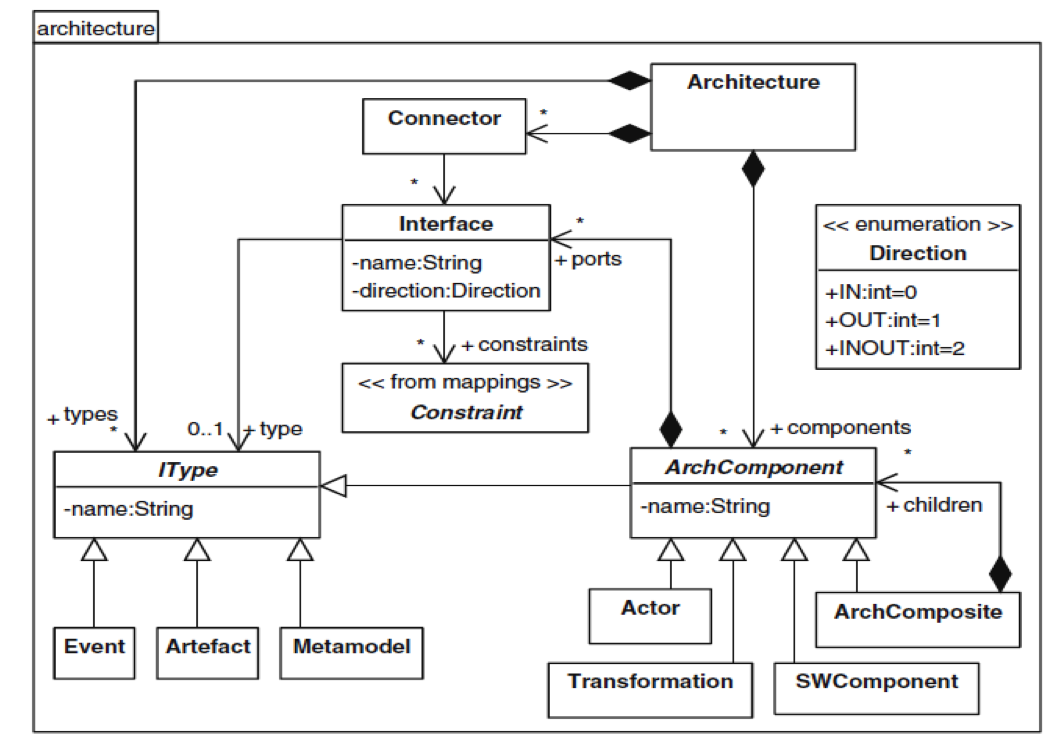
\includegraphics{transml-architecture.png}}}
\caption{\transml\ architecture metamodel}
\label{fig:transml-architecture}
\end{figure}

Constraints on interfaces can be used to impose a concept of contract, e.g., to restrict expected inputs and outputs, but also to support conformance checking.

Figure~\ref{fig:architecture-example1} shows an example of a unidirectional transformation architecture, using a simple component-based concrete syntax from UML. This example illustrates a transformation-centric view, i.e., the components in the architecture are themselves transformations. This can be contrasted with a type-centric architecture, shown in Figure~\ref{fig:architecture-example2}, where the components are types (or metamodels). In both cases, the example architecture is for a chain of transformations between an object-oriented model and SQL code.

\begin{figure}[htbp]
\centering{\scalebox{0.6}{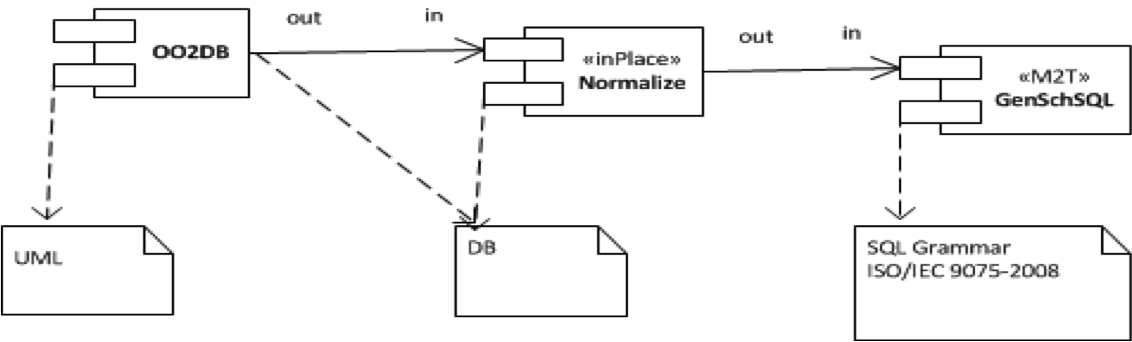
\includegraphics{transml-arch-example1.png}}}
\caption{\transml\ architecture example (transformation-centric)}
\label{fig:architecture-example1}
\end{figure}

In the above example, firstly a unidirectional OO2DB transformation is executed (taking a UML model as input and producing a DB model as output). Then, a normalising update-in-place transformation is executed on the DB model. Finally, a model-to-text transformation is executed on the DB model, producing SQL compliant to a specific grammar.

\begin{figure}[htbp]
\centering{\scalebox{0.6}{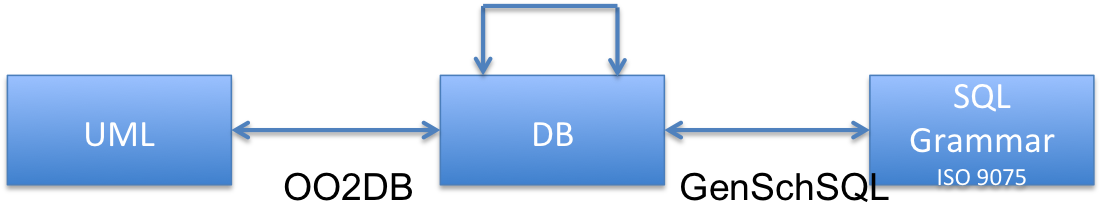
\includegraphics{transml-arch-example2.png}}}
\caption{\transml\ architecture example (type-centric, bidirectional)}
\label{fig:architecture-example2}
\end{figure}

The type-centric view represents the individual transformations as relationships between components. We have extended this example to represent bidirectional transformations throughout: i.e., the OO2DB, Normalise and GenSchSQL (the model-to-text transformation) could be executed in either direction.  We could, of course, present the same BX in a transformation-centric style. In this case, the architecture in Figure~\ref{fig:architecture-example1} would have bidirectional dependencies on the relevant input and output models, as depicted in Figure~\ref{fig:architecture-example3}.

\begin{figure}[htbp]
\centering{\scalebox{0.6}{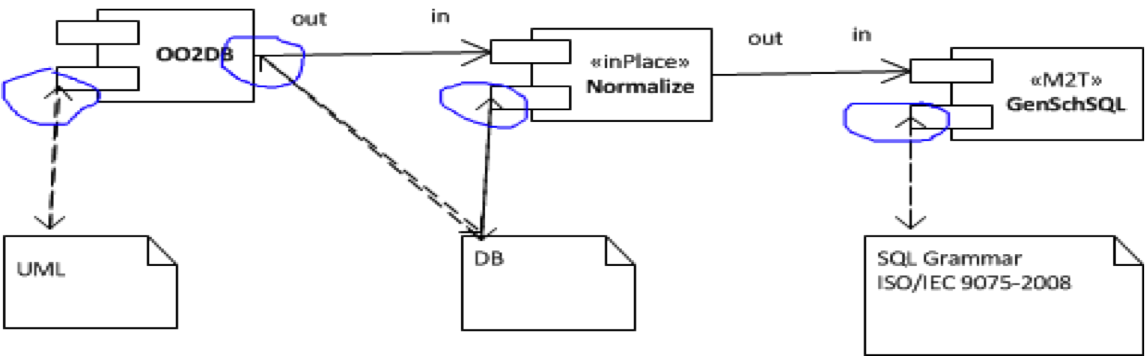
\includegraphics{transml-arch-example3.png}}}
\caption{\transml\ architecture example (transformation-centric, bidirectional)}
\label{fig:architecture-example3}
\end{figure}

\subsection{Design of BX}
The architecture of a software system captures the key components and their interrelationships. In the case of a BX this includes the connections between transformation components, the ports through which components communicate, and restrictions and constraints on that communication. The engineering process for BX continues with design, which can be broken into two parts: \textit{high-level design}, which focuses on capturing \textit{what is transformed into what}; and \textit{low-level design}, which focuses on capturing \textit{how} the transformation is to be carried out. We briefly consider \transml\ support for each aspect.

High-level design of a BX, once again, aims to capture what is transformed into what. To represent this, \transml\ introduces a \textit{mapping diagram}, inspired by triple graph grammars. These capture the mappings between arbitrary model elements involved in the transformation. However, mappings are not meant to be used as a implementation model -- specifically, they are not meant to be used as a tracing mechanism to guide the execution of code (this, as we will soon see, is the purpose of the low-level design features of \transml\).

The \transml\ metamodel for mapping diagrams is illustrated in Figure~\ref{fig:transml-mapping-diagram}. Mappings have ends which are associated with modelling elements. Navigability is a property of mappings; BX will involve navigation to both source and target. Constraints can be attached to mappings in order to define conditions on when (part of) a mapping can hold. 

\begin{figure}[htbp]
\centering{\scalebox{0.6}{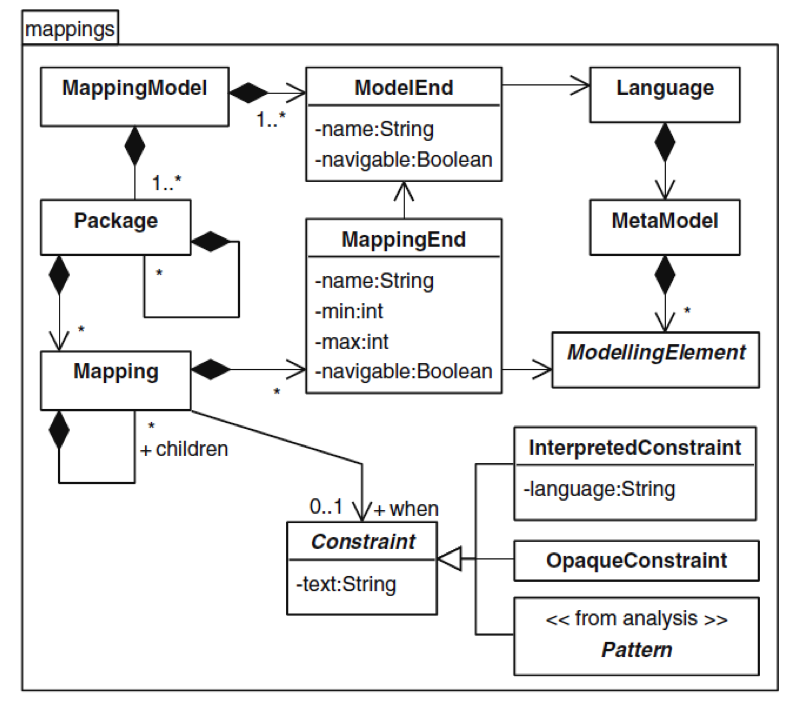
\includegraphics{transml-mapping-diagram.png}}}
\caption{\transml\ mapping diagram metamodel}
\label{fig:transml-mapping-diagram}
\end{figure}

Figure~\ref{fig:transml-mapping-example1} illustrates a mapping, for the Class2Relational BX. On the left of the diagram is a package containing key modelling elements of an OO model; on the right, a database model. In the centre are the mappings along with some informal English text explaining the purpose of each distinct mapping. Note the navigability of each rule; these can be executed from a DB model to an OO model, or vice versa.

\begin{figure}[htbp]
\centering{\scalebox{0.6}{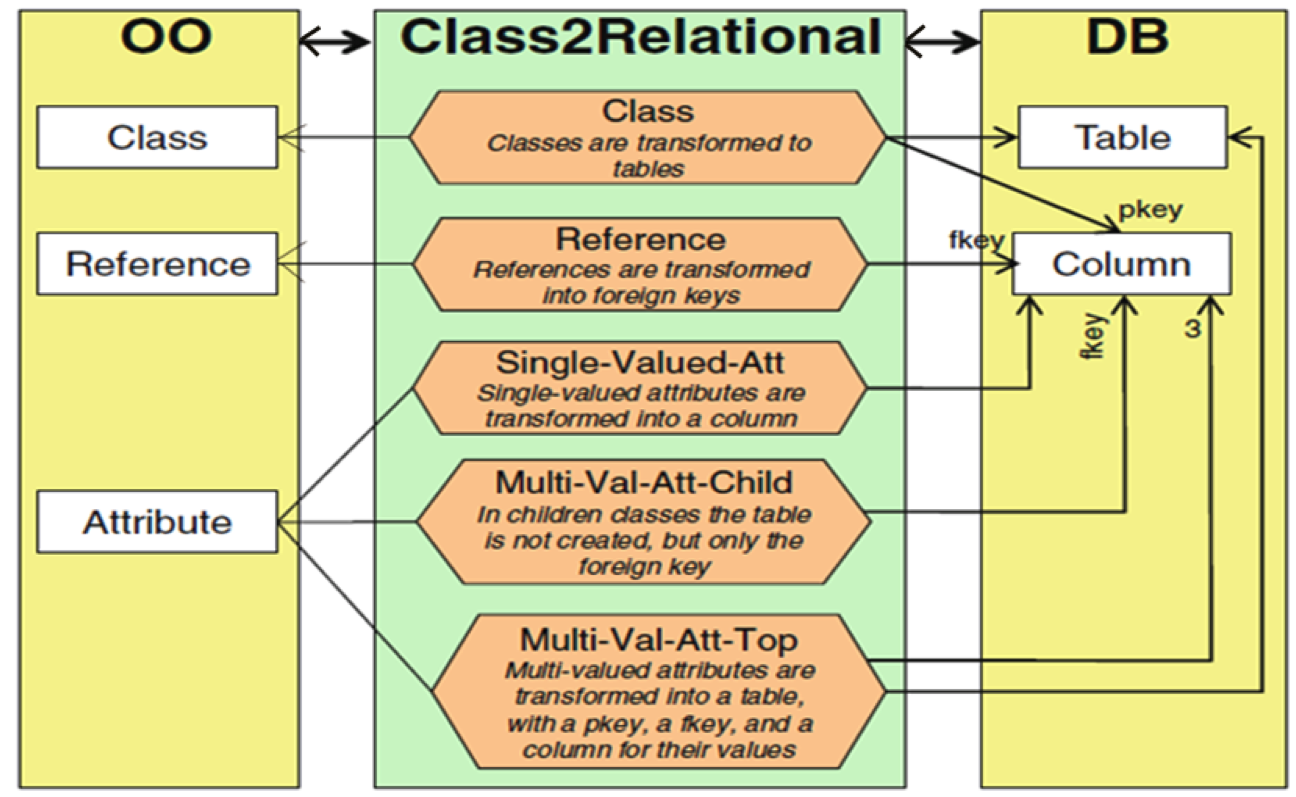
\includegraphics{transml-mapping-example1.png}}}
\caption{\transml\ mapping example}
\label{fig:transml-mapping-example1}
\end{figure}

The next example elaborates what is presented in Figure~\ref{fig:transml-mapping-example1} and imposes a constraint on the very last mapping, Multi-Val-Att-Top. The constraint, expressed in OCL, states that the owner of an attribute cannot have any parent classes; this is so that multi-valued attributes can be appropriately flattened into a table.

\begin{figure}[htbp]
\centering{\scalebox{0.6}{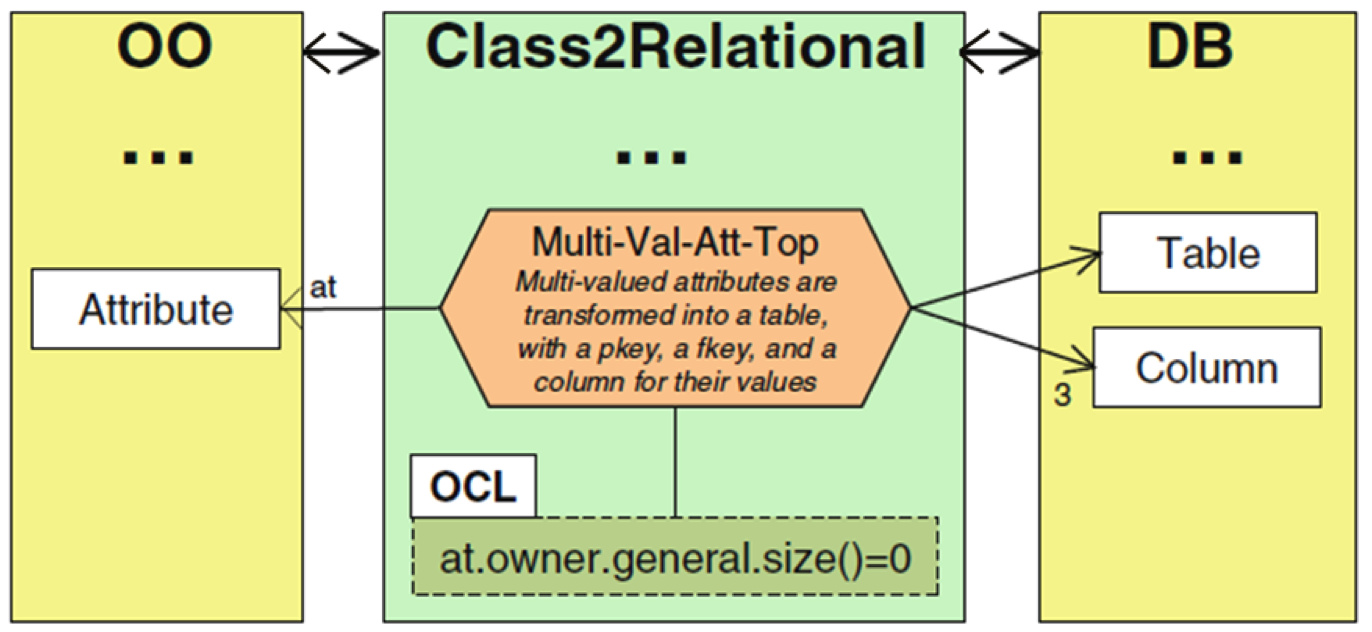
\includegraphics{transml-mapping-example2.png}}}
\caption{\transml\ mapping example (constraint)}
\label{fig:architecture-example3}
\end{figure}

While high-level design is supported in \transml\ via mapping diagrams, low-level design -- which is where the transition to implementation begins -- is
supported by more detailed diagrams. Technically, low-level design \textit{could} be supported by using a favourite BX programming language. But it may be preferable - for reasons of process - to maintain a degree of platform independence while still focusing on the essential aspects of BX development. As such, \transml\ provides low-level design languages for capturing the \textit{structure} of BX rules, control flow, and blocks. These are encapsulated in two diagrams: the \textit{rule structure diagram} and the \textit{rule behaviour diagram}.

The rule structure diagram (metamodel in Figure~\ref{fig:transml-rulestructure} is used to refine a mapping diagram. A rule can contribute to the implementation of one or more mappings. Rules themselves may be unidirectional or bidirectional. Structure diagrams also allow for explicit or implicit (e.g., nondeterministic) capture of execution flow, via subclasses of the \textit{Flow} metaclass. In particular, a set of rules can be placed inside a nondeterministic block, for example, as in graph transformation programs.


